\chapter{Uitwendige gegevensstructuren}
\begin{itemize}
    \item Als de grootte van de gegevens de capaciteit van het intern geheugen overschrijdt, moeten deze gegevens opgeslagen worden in extern geheugen.
    \item We willen dat woordenboekoperaties nog steeds efficiënt uitgevoerd worden.
    \item Een harde schijf is veel trager dan een processor.
    \item Daarom moet het aantal schijfoperaties geminimaliseerd worden.
\end{itemize}

\section{B-trees}
\begin{itemize}
    \item Uitwendige evenwichte zoekboom.
    \item Heeft een zeer kleine hoogte.
    \item Het aantal sleutels $n$ is wel zeer groot.
    \item Er worden dus meerdere kinderen per knoop opgeslagen.
    \item Knopen kunnen best een volledige schijfpagina benutten.
\end{itemize}

\subsection{Definitie}
\begin{itemize}
    \item Een B-tree heeft een orde $m$ waarbij $m > 2$, en wordt gedefinieerd als volgt:
    \begin{itemize}
        \item Elke inwendige knoop heeft minstens $\lceil m/2 \rceil$ en hoogstens $m$ kinderen. Deze kinderen zijn wijzers naar andere knopen die op het extern geheugen staan.
        \begin{itemize}
            \item De wortel is de uitzondering die hieraan niet voldoet.
            \begin{itemize}
                \item Is de wortel geen blad, dan bevat het minstens twee kinderen.
                \item Is de wortel een blad, en dus de enigste knoop in de B-tree, dan bevat het minstens één kind.
            \end{itemize}
            \item Elke inwendige knoop behalve de wortel is dus zeker steeds voor de helft opgevuld.
        \end{itemize}
        \item Elke inwendige knoop met $k + 1$ kinderen bevat $k$ sleutels ($k <= m$). 
        \item Elk blad bevat hoogstens $m - 1$ en minstens $\lceil m/2 \rceil - 1$  sleutels.
        \item Alle bladeren bevinden zich op hetzelfde niveau.
    \end{itemize}
    \item Elke knoop bevat het volgende:
    \begin{itemize}
        \item Een geheel getal $k$ dan het huidig aantal sleutels in de knoop aanduidt.
        \item Een tabel voor maximaal $m$ pointers naar de kinderen van de knoop.
        \item Een tabel voor maximaal $m - 1$ sleutels, die stijgend gerangschikt zijn.
        \begin{itemize}
            \item Er is ook een tabel die bijbehorende informatie per sleutel bijhoudt.
            \item De $k$ geordende sleutels van de inwendige knoop verdelen het sleutelbereik in $k + 1$ deelgebieden.
            \item De sleutels uit de deelboom van het $i$-de kind $c_i$ liggen tussen de sleutels $s_{i - 1}$ en $s_i$.
        \end{itemize} 
        \item Een logische waarde $b$ die aanduidt of de knoop een blad is of niet.
    \end{itemize}
    \item $2-3$ bomen ($m=3$) of $2-3-4$ bomen ($m=4$) zijn eenvoudige voorbeelden van B-trees. Normaal is $m$ wel groter.
\end{itemize}

\subsection{Eigenschappen}
\begin{itemize}
    \item Stel $g = \lceil m/2 \rceil$.
    \item Het minimaal aantal knopen voor een boom met hoogte $h$ is dan
    $$1 + 2 + 2g + \dots + 2g^{h - 1} = 1 + 2\sum_{i=0}^{h - 1}g^i = 1 + 2\bigg(\frac{g^h - 1}{g - 1}\bigg) $$
    \begin{itemize}
        \item Als de wortel een blad is, is dat de enigste knoop.
        \item Als de wortel geen blad is, heeft het minimum twee kinderen.
        \item Elk ander kind heeft minimum $g$ kinderen.
    \end{itemize}
    \item De hoogte is bijgevolg $O(\lg n)$.
    \begin{itemize}
        \item Elke knoop heeft minstens $g - 1$ sleutels, behalve de wortel, die er minstens één heeft.
        \begin{align*}
            & n \geq 1 + 2(g - 1)\bigg(\frac{g^h - 1}{g - 1} \bigg) \\
            \rightarrow \;& n \geq 2g^h - 1 \\
            \rightarrow \;& h \leq log_g\bigg(\frac{n+1}{2}\bigg)
        \end{align*}
    \end{itemize}
    \item Een B-tree met $n$ uniform verdeelde sleutels gebruikt ongeveer $\frac{n}{m\ln 2}$ schijfpaginas. 
\end{itemize}

\subsection{Woordenboekoperaties}

\subsubsection{Zoeken}
\begin{itemize}
    \item In elke knoop moet een meerwegsbeslissing genomen worden.
    \item De knoop moet eerst in het geheugen ingelezen worden.
    \item De sleutel wordt opgezocht in de gerangschikte tabel met sleutels.
    \begin{itemize}
        \item Normaal zou binair zoeken efficiënter zijn, maar deze winst is vrij onbelangrijk.
        \item Lineair zoeken kan bij kleine tabellen efficiënter uitvallen door het aantal cachefouten te minimaliseren.
    \end{itemize}
    \item Er kunnen zich nu drie situaties voordoen:
    \begin{enumerate}
        \item Als de sleutel in de tabel zit stopt het zoeken, met als resultaat een verwijzing naar de knoop op de schijf.
        \item Als de sleutel niet gevonden is en is de knoop een blad, dan zit de sleutel niet in de boom.
        \item Als de sleutel niet gevonden is en de knoop is inwendig, wordt een nieuwe knoop in het geheugen ingelezen waarvan de wortel een kind is van de huidige knoop. Het zoekproces start opnieuw met deze knoop.
    \end{enumerate}
    \item Performantie:
    \begin{itemize}
        \item Het aantal schijfoperaties is $O(h) = O(log_g n)$.
        \item De processortijd per knoop is $O(m)$.
        \item De totale performantie is $O(m\log_g n)$.
    \end{itemize}

\end{itemize}
\subsubsection{Toevoegen}
\begin{itemize}
    \item Toevoegen gebeurt \textbf{bottom-up}. Een top-down implementatie is ook mogelijk maar wordt minder gebruikt.
    \item De structuur van de boom kan gewijzigd worden.
    \item Toevoegen gebeurt altijd aan een blad.
    \item Vanuit de wortel wordt eerst het blad gezocht waarin de sleutel zou moeten zitten.
    \item Drie gevallen:
    \begin{enumerate}
        \item \textbf{De B-tree is ledig.}
        \begin{itemize}
            \item De wortelknoop wordt in het geheugen aangemaakt met de sleutel.
            \item De knoop wordt dan naar de schijf gekopieërd.
            \item De verwijzing naar de plaats van de wortel moet ook permanent bijgehouden worden.
        \end{itemize}
        \item \textbf{De B-tree is niet ledig.} Het blad waarin de sleutel moet zitten wordt opgezocht. Er zijn dan twee gevallen.
        \begin{enumerate}
            \item \textbf{Het blad bevat minder dan $m$ sleutels.}
            \begin{itemize}
                \item De sleutel wordt in de juiste volgorde toegevoegd aan de tabel met sleutels.
            \end{itemize}
            \item \textbf{Het blad bevat $m$ sleutels.} Er zijn dan twee manieren die gehanteerd kunnen worden:
            \begin{enumerate}
                \item De eerste manier splitst het blad op bij de middelste sleutel. Er wordt een nieuwe knoop aangemaakt op hetzelfde niveau, waarin de gegevens van rechts van de middelste sleutel terechtkomen. De middelste sleutel gaat dan naar zijn ouder, waar er eventueel opnieuw gesplitst kan worden.
                \item Een andere manier stelt het splitsen uit, door een rotatie uit te voeren. Als er een broer is die plaats heeft voor extra sleutels, kan die deze sleutels aannemen. Om de inorder volgorde van de sleutels te behouden wordt er eerst een sleutel aan de ouder gegeven, die een andere sleutel afstaat aan de gekozen broer.
            \end{enumerate}


        \end{enumerate}
    \end{enumerate}
    \item Performantie:
    \begin{itemize}
        \item In het slechtste geval worden er $h + 1$ knopen gesplitst. 
        \item Een knoop splitsen vereist drie schijfoperaties en een processortijd van $O(m)$.
        \item In het slechtste geval moet de boom tweemaal doorlopen worden.
        \begin{itemize}
            \item Eerst om de sleutel te vinden.
            \item Daarna eventueel tot de wortel splitsen.
            \good Maar het aantal schijfoperaties per niveau is constant.
        \end{itemize}
        \item Het totaal aantal schijfoperaties is $\Theta(h)$.
        \item De totale performantie is dan $O(mh) = O(m \log_g n)$.
    \end{itemize}
   
\end{itemize}

\subsubsection{Verwijderen}
\begin{itemize}
    \item Ook hier wordt enkel de \textbf{bottom-up} versie besproken.
    \item De gezochte sleutel kan zowel in een blad als in een inwendige knoop zitten.
    \begin{itemize}
        \item \textbf{De sleutel zit in een blad.}
        \begin{itemize}
            \item Er zijn geen kinderen meer dus kan de sleutel verwijderd worden.
            \item Het kan zijn dat het blad nu te weinig sleutels heeft (minder dan $\lceil m/2 \rceil - 1$).
            \item Er wordt een sleutel geleend van de ouder.
            \item In het slechtste geval gaat dit ontlenen door tot aan de wortel.
            \item Een sleutel ontlenen van een wortel die slechts één sleutel bevat maakt hem ledig, zodat de wortel verwijdert wordt.
        \end{itemize}
        \item \textbf{De sleutel zit in een inwendige knoop.}
        \begin{itemize}
            \item De sleutel wordt vervangen door zijn voorloper of opvolger, want die zitten zeker in een blad.
            \item De oorspronkelijke positie van de voorloper of opvolger wordt dan verwijdert uit het blad.
            \item Als een knoop nu te weinig sleutels overhoudt, gebeurt er een \textbf{rotatie}.
            \begin{itemize}
                \item Een sleutel van zijn broer gaat naar zijn ouder.
                \item Een sleutel van de ouder gaat naar de knoop, die ook een kindwijzer van de broer overneemt.
                \item Dit kan enkel als er een broer is die sleutels kan missen.
                \item Als geen enkele broer een sleutel kan missen, wordt de knoop samengevoegd met een broer.
            \end{itemize}
        \end{itemize}
    \end{itemize}
    \item Performantie:
    \begin{itemize}
        \item Analoog aan toevoegen en is dan $O(m\log_g n)$.
    \end{itemize}
\end{itemize}
\subsection{Varianten van B-trees}
\begin{itemize}
    \item Nadelen van een gewone B-tree:
    \begin{itemize}
        \item De bladeren moeten plaats reserveren voor kindwijzers die toch niet gebruikt worden.
        \item Inwendige knopen kunnen gegevens bevatten en dat maakt verwijderen veel ingewikkelder.
        \item Zoeken naar een opvolger van een sleutel kan $O(\log_g n)$ schijfoperaties vereisen.
    \end{itemize}
\end{itemize}
\subsubsection{$B^+$-tree}
\begin{itemize}
    \item Alle gegevens en bijhorende informatie zitten in de bladeren.
    \item Inwendige knopen worden gebruikt als index om de gegevens snel te lokaliseren.
    \item Bladeren en inwendige knopen hebben dus een verschillende structuur.
    \item Er is ook een \textbf{sequence set}, een gelinkte lijst van alle bladeren in stijgende sleutelvolgorde.
    \item De inwendige knopen moeten enkel sleutels bevatten en geen bijhorende informatie zodat de maximale graad groter is dan de bladeren.
    \item De bladeren moeten geen plaats reserveren voor kindwijzers, zodat ze meer gegevens kunnen bevatten.
\end{itemize}
\subsubsection{Prefix $B^+$-tree}
\begin{itemize}
    \item Een variant van een $B^+$-tree voor strings.
    \item Strings kunnen echter veel plaats innemen.
    \item Om twee deelbomen van elkaar te onderscheiden wordt de kleinst mogelijke prefix bijgehouden.
\end{itemize}
\subsubsection{$B^*$-tree}
\begin{itemize}
    \item In plaats van enkel gegevens over te brengen naar een buur tijdens het splitsen, worden de gegevens verdeeld over \textbf{drie} knopen.
    \item De wortel heeft geen buur, dus er wordt toegestaan dat de wortel tot $4/3$ gevuld kan worden, want dan kunnen twee knopen voor $2/3$ gevuld worden.
    \item Beter gevulde knopen betekent een minder hoge boom.
\end{itemize}
\section{Uitwendige hashing}
\begin{itemize}
    \item Waneer de volgorde van de sleutels niet belangreijk is.
    \item De woordenboekoperaties vereisen gemiddeld slechts $O(1)$.
    \item Er wordt een imaginaire binaire trie (hoofdstuk 10, figuur \ref{fig:binary_trie_hashing}) gebruikt.
    \begin{figure}[ht]
        \centering
        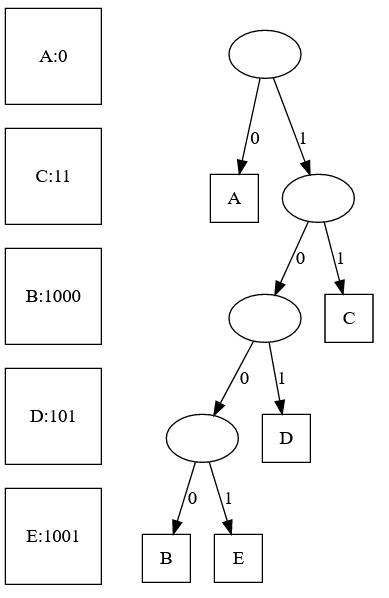
\includegraphics[width=0.3\textwidth]{binary_trie_hashing}
        \caption{Er zijn vijf schijfpagina's $A, B, C, D$ en $E$. Tijdens het hashen heeft elke pagina een hashwaarde gekregen, waarin sleutels met dezelfde hashwaarde ook in terechtkomen. De binaire trie laat toe om snel in een pagina te geraken door opeenvolgende bits te vergelijken van de hashwaarden.}
        \label{fig:binary_trie_hashing}
    \end{figure}
    \begin{itemize}
        \item Wanneer een sleutel gezocht wordt, worden de sleutels niet vergeleken maar wel de opeenvolgende bits van de sleutel.
        \item Elke deelboom van een trie bevat alle sleutels met een gemeenschappelijk prefix.
        \item Alle sleutels van een deelboom kan in één pagina ondergebracht worden.
        \item Als de pagina vol geraakt, wordt de knoop (en dus de pagina) gesplitst, en beide pagina's krijgen een nieuwe trieknoop als ouder.
        \item De vorm van een trie is enkel afhankelijk van de bits van de sleutels, dus een goede hashfunctie geeft voldoende garantie dat deze trie evenwichtig zal zijn.
    \end{itemize}
    \item Dit hoofdstuk bespreekt twee methoden: \textbf{extendible hashing} en \textbf{linear hashing} die beiden niet expliciet een trie gebruiken.

\end{itemize}

\subsection{Extendible hashing}
\begin{itemize}
    \item Er is een hashtabel in het geheugen.
    \item Het zoeken in de trie wordt geëlimineerd door de langst mogelijke prefix uit de trie als index te gebruiken in een hashtabel.
    \item Kortere prefixen komen overeen met meerdere tabelelementen die allemaal een verwijzing naar dezelfde pagina moet bevatten.
    \begin{itemize}
        \item De trie uit figuur \ref{fig:binary_trie_hashing} kan dus omgevormd worden in tabelvorm:
        \begin{table}[h]
            \centering
            \begin{tabular}{ | c | c |}
                \hline
                0000 & A \\
                0001 & A\\
                0010 & A\\
                0011 & A\\
                0100 & A\\
                0101 & A\\
                0110 & A\\
                0111 & A\\
                1000 & B\\
                1001 & E\\
                1010 & D\\
                1011 & D\\
                1100 & C\\
                1101 & C\\
                1110 & C\\
                1111 & C\\
                \hline
            \end{tabular}
            \caption{De tabelvorm van de boom uit figuur \ref{fig:binary_trie_hashing}. De eerste 8 elementen wijzen allemaal naar dezelfde pagina: $A$.}
        \end{table}
    \end{itemize}
    \item Implementatie:
    \begin{itemize}
        \item Er is een hashtabel die wijzers naar schijfpagina's bevat, waarbij elke schijfpagina maximaal $m$ sleutels met bijbehorende gegevens bevat.
        \item De hashwaarden zijn gehele getallen, waarvan het bereik bepaald wordt door de breedte $w$ van een processorwoord.
        \item Het prefix met lengte $d$ van die getallen dienen als indices in de hashtabel, zodat de tabel $2^d$ elementen bevat.
        \item De \textbf{globale diepte} is $d$ en is de lengte van het langste prefix in de trie.
        \item Alle sleutels waarvan de hashwaarde met dezelfde $d$ bits eindigt komen bij hetzelfde tabelelement terecht.
        \item Een pagina kan sleutels met hashwaarden bevatten waarvan de laatste $d$ bits verschillend zijn.
        \item Het aantal bits $k$ is de \textbf{lokale diepte} van een pagina en is de lengte van het aantal bits waarmee alle prefixen overeenkomen.
    \end{itemize}
    \item De \textbf{woordenboekoperaties:}
    \begin{itemize}
        \item \textbf{Zoeken.}
        \begin{itemize}
            \item Bereken de hashwaarde van de sleutel.
            \item Zoek de overeenkomstige pagina via de hashtabel.
            \item Zoek sequentieel in deze pagina.
        \end{itemize}
        \item \textbf{Toevoegen.}
        \begin{itemize}
            \item Als de pagina niet vol is moet gemiddeld helft van de elementen opgeschoven worden, maar dat is verwaarloosbaar.
            \item Als de pagina vol is moet deze gesplitst worden.
            \item Alle hashwaarden in die pagina beginnen met dezelfde $k$ bits.
            \item Er wordt daarom gesplitst op het volgende bit $k + 1$. Alle elementen in de pagina waarbij die bit één is wordt overgebracht naar de nieuwe pagina.
            \item De waarde van $k$ wordt één groter zowel in de nieuwe pagina als in de oude pagina.
            \item De hashtabel moet ook aangepast worden.
            \begin{itemize}
                \item \textbf{Als $k$ kleiner was dan $d$:} de helft van de wijzers van de oude pagina moeten naar de nieuwe pagina wijzen.
                \item \textbf{Als $k$ gelijk was aan $d$:} er was maar één wijzer naar de oude pagina. De waarde van $d$ moet ook met één toenemen en de grootte van de hashtabel moet \textbf{verdubbelt} worden.
            \end{itemize}           
        \end{itemize}
        \item \textbf{Verwijderen.}
        \begin{itemize}
            \item Als een pagina en haar ooit afgesplitste buur samen minder dan $m$ sleutels bevatten kan men ze samenvoegen.
            \item Er verdwijnt een pagina en het hashtabelelement moet naar de andere pagina wijzen waarvan $k$ met één verminder wordt.
            \item Als de hashtabel minstens twee verwijzingen naar elke pagina bevat (elke $k$ is kleiner dan $d$) kan de tabel gehalveerd worden.
        \end{itemize}
    \end{itemize}
    \item Als er $n$ uniform verdeelde sleutels opgeslagen zijn, dan is de verwachtingswaarde van het aantal pagina's $n/(m\ln 2) \equiv 1.44n/m$.
    
\end{itemize}

\subsection{Linear hashing}
\begin{itemize}
    \item Er wordt geen hashtabel gebruikt door ervoor te zorgen dat pagina's opeenvolgende adressen hebben.
    \item De $d$ eindbits van de hashwaarde worden niet gebruikt als index, maar rechtstreeks als adres van een pagina.
    \item Het gaat hier over \textbf{logische adressen}, die eenvoudig manipuleerbaar zijn en niet de \textbf{fysische adressen} die het besturingssysteem beheert.
    \item Er zijn $2^d$ adressen en evenveel pagina's.
    \item Als een pagina vol is wordt deze gesplitst, maar niet noodzakelijk de hele pagina.
    \item Pagina's worden in sequentiële volgorde gesplitst, of ze nu vol zijn of niet.
    \item Elke pagina die niet vol is (alle pagina's behalve de volle die het splitsen veroorzaakt heeft) krijgt een overflow pagina.
    \item Als de pagina aan de beurt is om te splitsen, worden zijn gegevens verdeeld over zijn overflow pagina en de pagina zelf.
    \item De \textbf{woordenboekoperaties:} 
    \begin{itemize}
        \item \textbf{Zoeken.}
        \begin{itemize}
            \item Bereken de hashwaarde van de sleutel.
            \item We moeten echter weten hoeveel eindbits er nodig zijn om de pagina te adresseren.
            \item Er wordt een variabele $p$ bijgehouden, die het adres van de volgende te splitsen pagina bijhoudt.
            \item Het adres gevormd door de $d$ eindbits wordt vergeleken met $p$. 
            \item Als $d < p$ dan is de gezochte pagina reeds gesplitst en moeten $d + 1$ eindbits gebruikt worden. Anders volstaan $d$ bits.
            \item De sleutel kan in de pagina binair of lineair gezocht worden.
        \end{itemize}
        \item \textbf{Toevoegen.}
        \begin{itemize}
            \item Eerst wordt de juiste pagina gelokaliseerd.
            \item Als de pagina vol zit moet ze gesplitst worden.
            \item Splitsen gebeurt sequentieël zodat $p = 0$ in het begin.
            \item $p$ wordt met één verhoogd tot alle $2^d$ pagina's gesplitst zijn.
            \item De waarde van $d$ wordt dan verhoogd met één, en $p$ wordt terug 0.
            \item Als pagina $p$ gesplitst wordt, is het adres van de nieuwe pagina $p + 2^d$.
        \end{itemize}
        \item \textbf{Verwijderen.}
        \begin{itemize}
            \item Lokaliseer de pagina.
            \item Verwijder het gegeven uit de tabel van die pagina.
            \item Onderbezette pagina's verwijden in omgekeerde volgorde als waarin ze gecreëerd werden.
        \end{itemize}
    \end{itemize}                                                                                                                                                           
\end{itemize}